\subsection{Tubular Segmentation plugin}

This plugin adds a new interactive way of defining segmentations. The user creates a
segmentation by defining a list of spheres (centers and radious) in the three-dimensional
space of the sample, that will be later connected with tubes.
That way a tubular segmentation is created.\\

\begin{figure}[H]
\centering
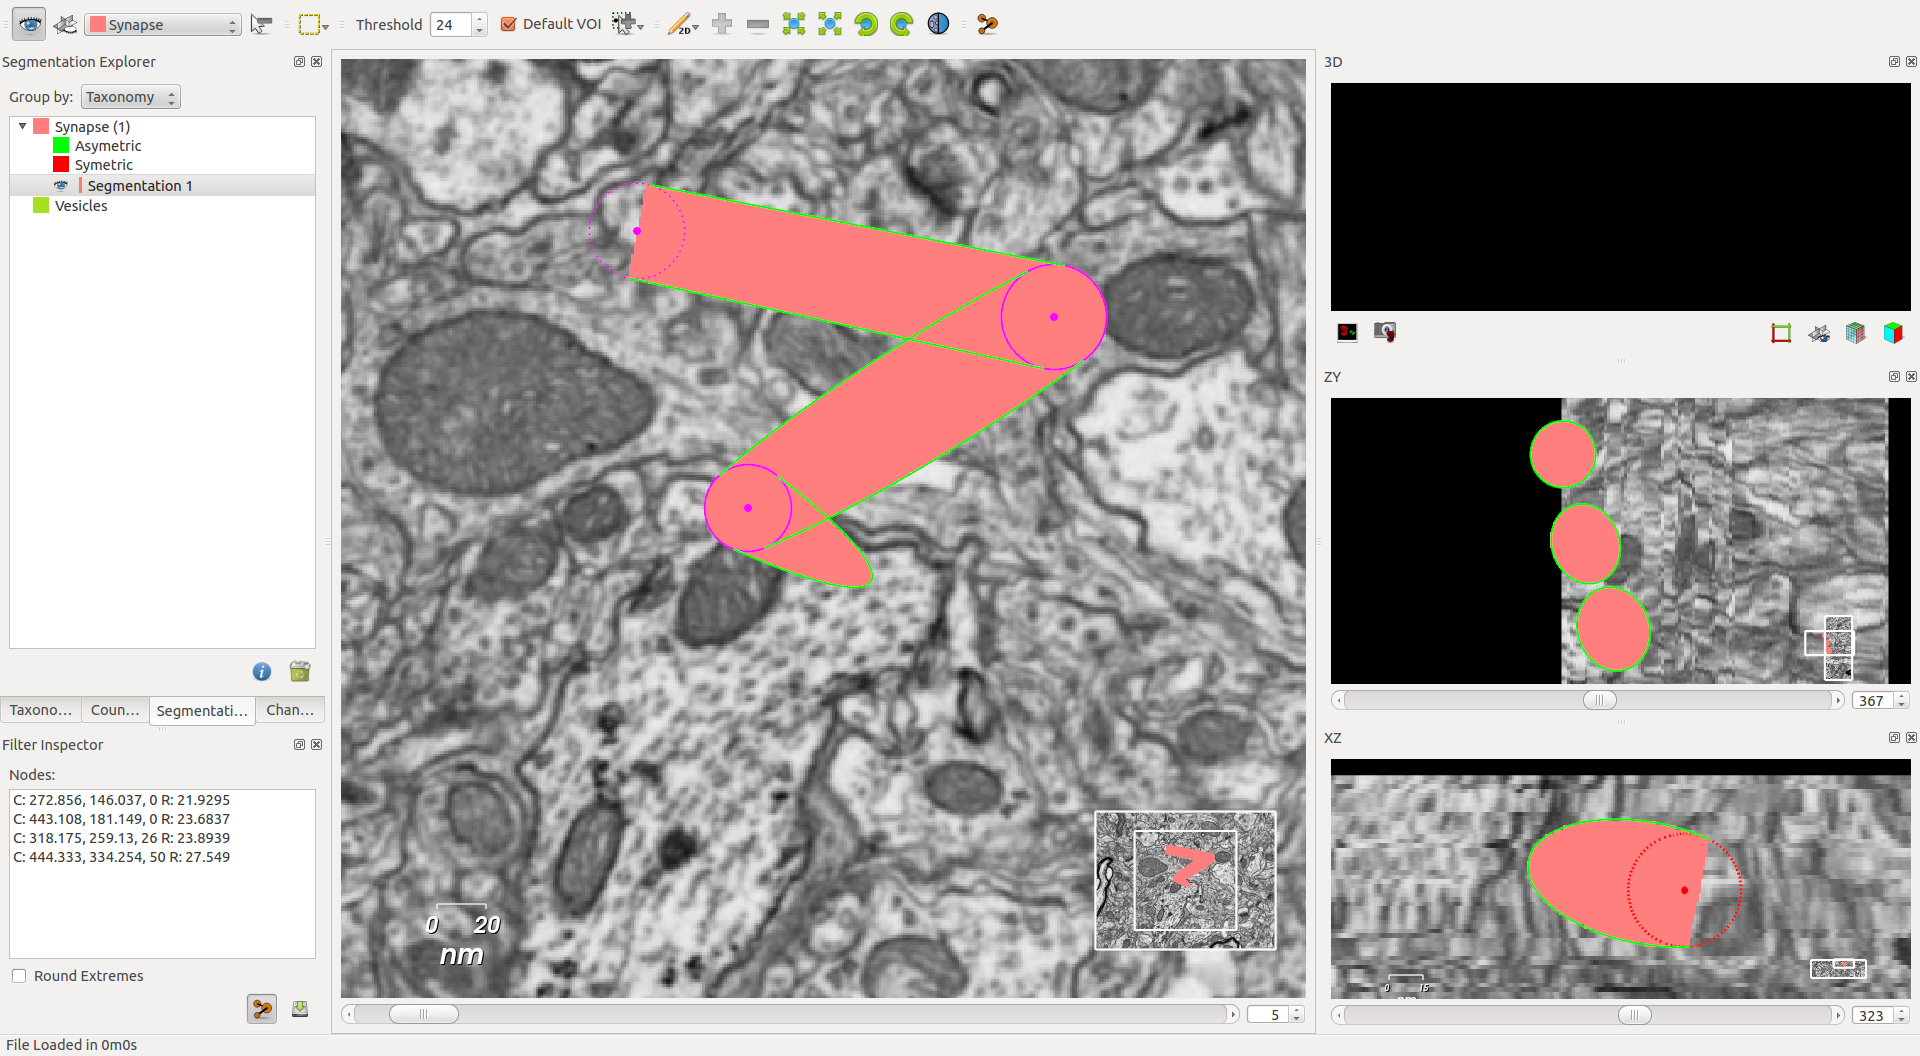
\includegraphics[scale=0.2]{fig/plugin-ts-segmentation.png}
\caption{A tubular segmentation with flat extremes.}
\end{figure}

To create a tubular segmentation use the associated toolbar. The toolbar is used to \textbf{create} a
new segmentation. To \textbf{modify} an existing segmentation the user must use a similar button located
in the filter inspector.
 
\begin{figure}[H]
\centering

\includegraphics[scale=0.75]{fig/plugin-ts-toolbar.png}
\caption{Tubular segmentations toolbar.}
\end{figure}

\begin{tabular}{| m{1.3cm} | m{12cm} |}
\hline
\textbf{Button} & \textbf{Description}\\
\hline

\includegraphics[width=0.7cm]{fig/tubular} & Create a new tubular segmentation.\\
\hline
\end{tabular}
\vspace{0.3cm} 

To create a segmentation the user must click on the screen to define a sphere centen and, once the center
has been defined, a sphere border will be created. The user must then define the length of the radius of the 
sphere by clicking on the screen again when it has reached the desired lenght. To place the next sphere in
the tubular segmentation the user must repeat the process used to create the first. When the next sphere has
been defined the interface will show the tube that joins both spheres, and so on. \\
By default the newly created segmentation won't have it's extremes rounded, that is shown during creation by
drawing the first and last spheres with a discontinuous border, while the rest of the spheres will have a
solid border. This behaviour can be changed in the filter inspector. \\

In the filter inspector widget of a tubular segmentation the nodes that define the segmentation are shown.\\

\begin{figure}[H]
\centering
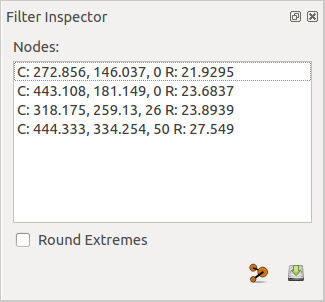
\includegraphics[scale=0.75]{fig/plugin-ts-inspector.png}
\caption{Tubular segmentations toolbar.}
\end{figure}

\begin{tabular}{| m{1.3cm} | m{12cm} |}
\hline
\textbf{Button} & \textbf{Description}\\
\hline
Nodes & Node list with the coordinates of the center of the node and it's radius.\\
\hline

\includegraphics[width=0.7cm]{fig/tubular} & Modify the nodes that define this segmentation.\\
\hline
Save & Save the node list to a text file.\\
\hline
Round Extremes & Toggles between rounded/flat extremes segmentations.\\
\hline
\end{tabular}
\vspace{0.3cm} 

